\subsection{Qualità di processo - Documentazione}

\subsubsection{Errori Ortografici}
\begin{figure}[H]
    \centering
    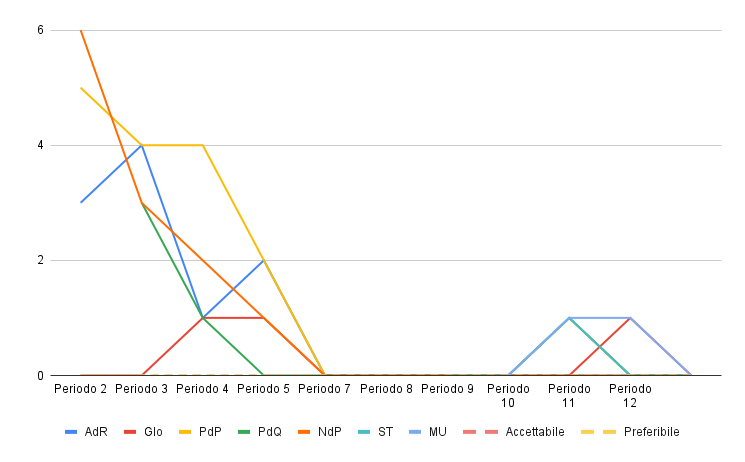
\includegraphics[width=0.8\textwidth]{../Images/PianoDiQualifica/errori_ortografici.png}
    \caption{Resoconto errori ortografici}
    \label{fig:Errori ortografici}
\end{figure}

\textbf{RTB}: Il grafico mostra l'andamento degli errori ortografici rilevati nei documenti. Si nota come il numero di errori ortografici sia inizialmente alto, ma tenda a diminuire con l'avanzare del progetto. Questo è dovuto al fatto che il gruppo ha iniziato a prestare maggiore attenzione alla scrittura dei documenti raggiugendo l'ottimo nell'ultimo periodo.

\subsubsection{Indice di Gulpease}
\begin{figure}[H]
    \centering
    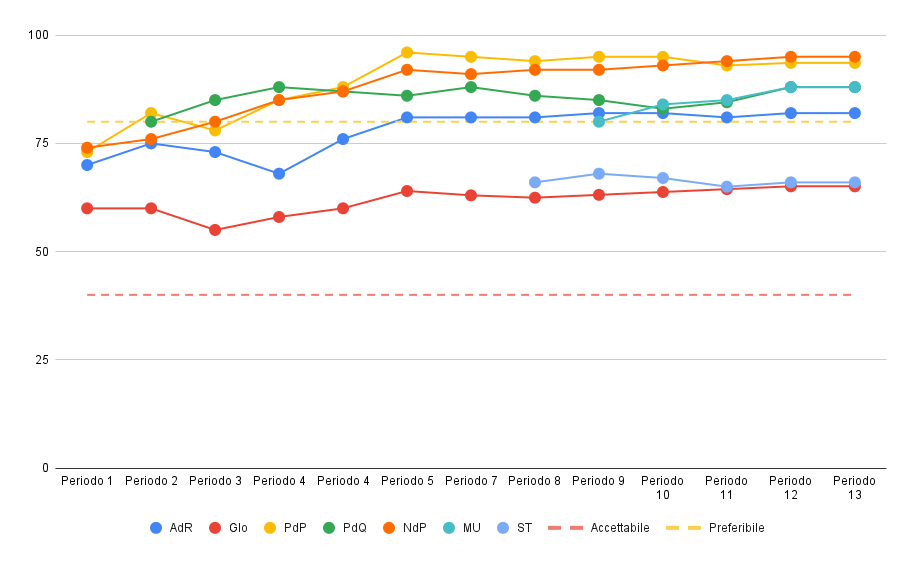
\includegraphics[width=0.8\textwidth]{../Images/PianoDiQualifica/Gulpease.png}
    \caption{Resoconto indice di Gulpease}
    \label{fig:Indice di Gulpease}
\end{figure}